% !TeX program = xelatex
% 统一模板：A4、中文宋体、五号（10.5 pt）、XeLaTeX 编译。
% 本前导区完整内嵌于每一份试卷，试卷之间没有相互依赖。
\documentclass[UTF8,zihao=5,fontset=none,a4paper]{ctexart}
\IfFontExistsTF{SimSun}{%
  \setCJKmainfont{SimSun}[BoldFont=SimHei,ItalicFont=KaiTi]
  \setCJKsansfont{SimHei}
  \setCJKmonofont{FangSong}
}{%
  \setCJKmainfont{FandolSong-Regular}[BoldFont=FandolSong-Bold,ItalicFont=FandolKai-Regular]
  \setCJKsansfont{FandolHei-Regular}
  \setCJKmonofont{FandolFang-Regular}
}
\usepackage[left=23mm,right=23mm,top=23mm,bottom=23mm,headheight=15pt]{geometry}
\usepackage{amsmath,amssymb,bm}
\usepackage{graphicx,array,tabularx,enumitem,needspace}
\usepackage{tikz}
\usetikzlibrary{arrows.meta,decorations.pathmorphing,patterns,calc,angles,quotes}
\usepackage{fancyhdr,lastpage}
\usepackage[hidelinks,unicode]{hyperref}
\setlength{\parindent}{0pt}
\setlength{\parskip}{4pt}
\linespread{1.22}
\setlength{\emergencystretch}{2em}
\setlength{\abovedisplayskip}{6pt}
\setlength{\belowdisplayskip}{6pt}
\setlist[enumerate]{leftmargin=2em,itemsep=3pt,topsep=3pt}
\ctexset{section={format=\zihao{5}\bfseries,number={},beforeskip=12pt,afterskip=6pt}}
\pagestyle{fancy}
\fancyhf{}
\fancyhead[L]{\zihao{5}\ExamShort}
\fancyhead[R]{\zihao{5}大学物理 BII}
\fancyfoot[C]{\zihao{5}第 \thepage\ 页\quad 共 \pageref*{LastPage}\ 页}
\renewcommand{\headrulewidth}{0.4pt}
\newcommand{\makexamtitle}{%
  \begin{center}\zihao{5}\bfseries\ExamTitle\end{center}\vspace{3pt}}
\newcounter{question}
\newcommand{\q}{\par\Needspace{5\baselineskip}\refstepcounter{question}%
  \noindent\textbf{\thequestion、}\ignorespaces}
\newcommand{\resetquestions}{\setcounter{question}{0}}
\newcommand{\choices}[4]{\par\nopagebreak
  \begin{tabularx}{\linewidth}{@{}*{4}{>{\raggedright\arraybackslash}X}@{}}
  A.\ #1 & B.\ #2 & C.\ #3 & D.\ #4
  \end{tabularx}\par}
\newcommand{\choicestwo}[4]{\par\nopagebreak
  \begin{tabularx}{\linewidth}{@{}*{2}{>{\raggedright\arraybackslash}X}@{}}
  A.\ #1 & B.\ #2\\[5pt] C.\ #3 & D.\ #4
  \end{tabularx}\par}
\newcommand{\choiceslong}[4]{\par\nopagebreak
  \begin{enumerate}[label=\Alph*.,leftmargin=1.8em]
  \item #1 \item #2 \item #3 \item #4
  \end{enumerate}}
\newcommand{\choicesthree}[3]{\par\nopagebreak
  \begin{enumerate}[label=\Alph*.,leftmargin=1.8em]
  \item #1 \item #2 \item #3
  \end{enumerate}}
\newcommand{\blank}[1][2cm]{\underline{\hspace{#1}}}
\newcommand{\ans}[2]{\par\Needspace{4\baselineskip}\textbf{#1、#2}\par}
\newenvironment{diagram}{\par\nopagebreak\begin{center}%
  \begin{tikzpicture}[>=Stealth,line width=.65pt,font=\normalsize]}
  {\end{tikzpicture}\end{center}}
\newcommand{\figlabel}[1]{\par\nopagebreak{\centering #1\par}}
\newenvironment{questionblock}{\par\addvspace{5pt}\noindent
  \begin{minipage}{\linewidth}\setlength{\parskip}{4pt}}
  {\end{minipage}\par\addvspace{5pt}}
\tikzset{spring/.style={decorate,decoration={coil,aspect=.5,segment length=5pt,amplitude=4pt}},
  wall/.style={pattern=north east lines,pattern color=black}}

\newcommand{\ExamTitle}{东南大学2023--2024学年大学物理BII第二次月考试卷}
\newcommand{\ExamShort}{2023--2024学年\quad 第二次月考}
\hypersetup{pdftitle={东南大学2023—2024学年大学物理BII第二次月考试卷}}
\begin{document}
\makexamtitle
\begin{center}第一学期\end{center}
\begin{questionblock}
\section{一、选择题}
\q 真空中波长为 $\lambda$ 的单色光，在折射率为 $n$ 的大块玻璃中沿直线从 A 点经过路程 $l$ 到达 B 点，则 A、B 两点处光振动的相位差 $\Delta\varphi$ 为（\quad）。
\choices{$\Delta\varphi=\frac{2\pi nl}{\lambda}$}{$\Delta\varphi=\frac{2\pi l}{\lambda}$}
{$\Delta\varphi=\frac{2\pi l}{n\lambda}$}{$\Delta\varphi=\frac{2\pi n\lambda}{l}$}
\end{questionblock}
\begin{questionblock}
\q 在杨氏双缝干涉实验中，若单色光源 S 到两缝 $S_1$、$S_2$ 距离相等，则观察屏上中央明纹中心位于 $o$ 处，若将光源 S 向下移动到图中 $S'$ 位置，且 $S_1S'-S_2S'=3\lambda$，则（\quad）。
\begin{diagram}
\draw (-1,-.9)--(-1,.65);
\draw (0,-.95)--(0,-.55) (0,-.4)--(0,.4) (0,.55)--(0,1);
\draw (4,-.8)--(4,1.7);
\coordinate (S) at (-1,0);
\coordinate (A) at (0,.48); \coordinate (B) at (0,-.48);
\coordinate (P) at (4,1.35);
\draw (S)--(A)--(P) (S)--(B)--(P);
\draw[dotted] (S)--(P);
\draw (S)--(4,0);
\draw[dashed] (-1,-.5)--(A) (-1,-.5)--(B);
\node[left] at (S){S}; \node[left] at (-1,-.5){$S'$};
\node[above left] at (A){$S_1$}; \node[below left] at (B){$S_2$};
\node[right] at (P){P}; \node[below right] at (4,0){$o$};
\draw (.7,0) arc[start angle=0,end angle=15,radius=1.7];
\node at (1.1,.2){$\theta$};
\end{diagram}
\choiceslong{中央明纹中心向下移动至原来第 3 条暗纹中心的位置处，且条纹间距增大}
{中央明纹中心向下移动至原来第 3 级明纹中心的位置处，且条纹间距不变}
{中央明纹中心向上移动至原来第 3 条暗纹中心的位置处，且条纹间距减小}
{中央明纹中心向上移动至原来第 3 级明纹中心的位置处，且条纹间距不变}
\end{questionblock}
\begin{questionblock}
\q 为了测定空气折射率，在迈克耳孙干涉仪的一个臂上，放置有长度为 $l$ 的密封玻璃管，管内充以 1 个大气压的空气。设使用的单色光波长为 $\lambda$，现用真空泵将玻璃管中的空气逐渐抽出，观察到恰有 $N$ 条干涉明纹从视场中移过，则在 1 个大气压下的空气折射率为（\quad）。
\choices{$n=\frac{N\lambda}l+1$}{$n=\frac{N\lambda}l$}
{$n=\frac{N\lambda}{2l}+1$}{$n=\frac{N\lambda}{2l}$}
\end{questionblock}
\begin{questionblock}
\q 在双缝干涉实验中，观察屏上的 P 点是明纹中心。若将 $S_2$ 缝盖住，并在 $S_1S_2$ 连线的垂直平分面处放一反射镜 M（如图所示），则以下说法正确的是（\quad）。
\begin{diagram}
\draw (0,-1.1)--(0,-.7) (0,-.5)--(0,.5) (0,.7)--(0,1.1);
\draw (3.5,-1.1)--(3.5,2);
\fill[gray!35] (0,-.06) rectangle (2,.06);
\draw[thick] (0,.06)--(2,.06);
\draw (0,.6)--(3.5,1.7) node[midway,above]{$r_1$};
\draw (0,.6)--(1,0)--(3.5,1.7) node[midway,below]{$r_2$};
\draw[dashed] (0,-.6)--(1,0);
\node[left] at (0,.6){$S_1$}; \node[left] at (0,-.6){$S_2$};
\node[right] at (3.5,1.7){P}; \node[below] at (.9,-.15){M};
\end{diagram}
\choicestwo{P 点处仍为明纹中心}{P 点处变为暗纹中心}
{P 点处亮度变为原来的一半}{P 点处明或暗都有可能}
\end{questionblock}
\begin{questionblock}
\q 在双缝干涉实验中，两缝间距为 $0.30\,\mathrm{mm}$，用单色光垂直照射双缝，在离缝 $1.20\,\mathrm m$ 的屏上测得中央明纹一侧第 5 条暗纹与另一侧的第 5 条暗纹间的距离为 $22.78\,\mathrm{mm}$，则所用光的波长最接近以下的（\quad）。
\choices{$633\,\mathrm{nm}$}{$518\,\mathrm{nm}$}{$570\,\mathrm{nm}$}{$712\,\mathrm{nm}$}
\end{questionblock}
\begin{questionblock}
\q 如图所示，波长为 $\lambda$ 的电磁波垂直射到墙上，墙上有两个小孔 A 和 B，彼此相距 $a=4\lambda$，一个电磁波探测器从 A 出发，沿与墙垂直的直线 AP 向右移动，在 Q 点处第 1 次测到信号极大，则 Q 与 A 的距离为（\quad）。
\begin{diagram}
\draw[thick] (0,1.1)--(0,.1) (0,-.1)--(0,-1.4) (0,-1.6)--(0,-2.2);
\foreach \y in {.6,0,-.75,-1.5}{\draw[->] (-1.7,\y)--(-.15,\y);}
\node[align=center] at (-2.1,-.5){电\\磁\\波};
\draw[->] (0,0)--(2.7,0);
\node[above right] at (0,0){A}; \node[right] at (0,-1.5){B};
\node[right] at (0,-.75){$a$};
\fill (1,0) circle(2pt) node[above]{Q}; \node[above] at (2.4,0){P};
\end{diagram}
\choicesthree{$\frac54\lambda$}{$\frac76\lambda$}{$\lambda$}
\end{questionblock}
\begin{questionblock}
\q 集成光学中的楔形薄膜耦合器原理如图所示。氧化钽（$\mathrm{Ta_2O_5}$）薄膜沉积在玻璃衬底上，其楔形端从 A 到 B 厚度逐渐减小为零，倾角很小。薄膜的厚度为 $1.40\,\mu\mathrm m$，用波长 $\lambda=598\,\mathrm{nm}$ 的单色平行光沿入射角为 $30^\circ$ 角的方向射在膜的上表面，玻璃和 $\mathrm{Ta_2O_5}$ 对该光的折射率分别为 1.5 和 2.2，则反射光在楔形端形成的暗条纹中心的数目为（\quad）。
\begin{diagram}
\draw[fill=gray!45] (0,-.55) rectangle (3.3,0);
\draw[fill=gray!10] (0,0)--(0,.8)--(.8,.8)--(2.65,0)--cycle;
\draw[dashed] (.8,0)--(.8,.8);
\node[above] at (.8,.8){A}; \node[above right] at (2.65,0){B};
\end{diagram}
\choices{9}{11}{18}{22}
\end{questionblock}
\begin{questionblock}
\q 如图两块平玻璃构成空气劈尖，左边为棱边，用单色平行光垂直入射。若上面的平玻璃慢慢地向上平移，则干涉条纹（\quad）。
\begin{diagram}
\draw (0,0) rectangle (4,-.45);
\draw (0,0)--(4,.8)--(4,1.2)--(0,.4)--cycle;
\draw[dashed] (0,.55)--(4,1.35)--(4,1.75)--(0,.95)--cycle;
\draw[->,thick] (4.25,.85)--(4.25,1.75);
\end{diagram}
\choicestwo{向棱边方向平移，条纹间隔变小}{向棱边方向平移，条纹间隔变大}
{向棱边方向平移，条纹间隔不变}{向远离棱边的方向平移，条纹间隔不变}
\end{questionblock}
\begin{questionblock}
\q 如图所示，两个直径有微小差别的彼此平行的滚柱之间的距离为 $L$，夹在两块平板玻璃的中间，形成一空气劈尖，当单色光垂直入射时，产生等厚干涉条纹。如果让两滚柱之间的距离 $L$ 稍微变小，则在 $L$ 范围内干涉条纹的（\quad）。
\begin{diagram}
\draw (0,0) rectangle (4,-.35);
\draw (.65,.3) circle(.3); \draw (3.25,.44) circle(.44);
\draw (0,.53)--(4,.97)--(4,1.3)--(0,.86)--cycle;
\foreach \x in {1,1.8,2.6}{\draw[->] (\x,2.1)--(\x,1.45);}
\node at (2.1,2.1){$\lambda$};
\draw (.65,.3)--(.65,-.95) (3.25,.44)--(3.25,-.95);
\draw[<->] (.65,-.75)--(3.25,-.75) node[midway,below]{$L$};
\end{diagram}
\choicestwo{数目减少，间距变大}{数目减少，间距不变}
{数目不变，间距变小}{数目增加，间距变小}
\end{questionblock}
\begin{questionblock}
\q 如图所示，厚度为 $e$ 的透明介质薄膜折射率为 $n_2$，其上方和下方的透明介质的折射率分别为 $n_1$ 和 $n_3$，且 $n_1<n_2$、$n_2>n_3$，若用单色平行光垂直入射到该薄膜上，已知该单色光在介质薄膜中的波长为 $\lambda$，则从该薄膜上、下两表面反射的两光束的光程差可表示为（\quad）。
\begin{diagram}
\draw (0,0) rectangle (3,.8);
\node at (.35,1.15){$n_1$}; \node at (.35,.4){$n_2$}; \node at (.35,-.35){$n_3$};
\draw[->] (1.2,1.7)--(1.2,.8);
\draw[->] (1.2,.8)--(1.2,0);
\draw[->] (1.55,0)--(1.55,1.7);
\draw[->] (1.9,.8)--(1.9,1.7);
\draw[<->] (3.3,0)--(3.3,.8) node[midway,right]{$e$};
\end{diagram}
\choicesthree{$2n_2e$}{$2n_2e-\frac\lambda2$}{$2n_2e-\frac{n_2\lambda}2$}
\end{questionblock}
\begin{questionblock}
\q 把一平凸透镜放在平玻璃上，构成牛顿环装置。当平凸透镜慢慢地向上平移时，由反射光形成的牛顿环（\quad）。
\begin{diagram}
\draw (-1.5,-.45) rectangle (1.5,-.7);
\draw (-1.4,.1)--(1.4,.1) .. controls (.9,-.633) and (-.9,-.633) .. (-1.4,.1);
\foreach \x in {-1.1,-.65,-.2,.25,.7}{\draw[->] (\x,.9)--(\x,.18);}
\node at (-.2,1.15){$\lambda$};
\draw[->] (1.45,.2)--(1.45,.9);
\end{diagram}
\choicestwo{向中心收缩，条纹间隔变小}{向中心收缩，环心呈明暗交替变化}
{向外扩张，环心呈明暗交替变化}{向外扩张，条纹间隔变大}
\end{questionblock}
\begin{questionblock}
\q 如图所示，折射率 $n_2=1.2$ 的油滴落在折射率 $n_3=1.5$ 的平板玻璃上，形成一上表面近似于球面的油膜。已知空气的折射率 $n_1=1.0$，测得油膜中心最高处的高度 $d_{\mathrm m}=1.0\,\mu\mathrm m$，用 $\lambda=600\,\mathrm{nm}$ 的单色光垂直照射油膜，则关于反射光下面说法正确的是（\quad）。
\begin{diagram}
\draw[fill=gray!15] (-1.6,-.35) rectangle (1.6,0);
\draw[fill=gray!30] (-1.5,0) .. controls (-.5,.6) and (.5,.6) .. (1.5,0)--cycle;
\foreach \x in {-1,-.5,0,.5,1}{\draw[->] (\x,1.6)--(\x,.75);}
\node at (.2,1.45){$\lambda$};
\node at (-1.25,.5){$n_1$}; \node at (-.6,.15){$n_2$}; \node at (-1.25,-.18){$n_3$};
\draw[thin] (0,.45)--(1.85,.45) (1.6,0)--(1.85,0);
\draw[<->] (1.75,0)--(1.75,.45) node[midway,right]{$d_{\mathrm m}$};
\end{diagram}
\choicestwo{干涉条纹内密外疏，有 4 个暗环}{干涉条纹内密外疏，有 5 个暗环}
{干涉条纹内疏外密，有 4 个暗环}{干涉条纹内疏外密，有 5 个暗环}
\end{questionblock}
\begin{questionblock}
\q 已知地球到月球的距离是 $3.84\times10^8\,\mathrm m$，云南天文台丽江观测站有一 $2.4\,\mathrm m$ 口径的天文望远镜，若用此望远镜观察月球表面时，刚好将月球正面一环形山上的两点分辨开，则该两点的距离为（设接收到来自月球的光的波长为 $600\,\mathrm{nm}$）（\quad）。
\choices{$181\,\mathrm m$}{$281\,\mathrm m$}{$234\,\mathrm m$}{$117\,\mathrm m$}
\end{questionblock}
\begin{questionblock}
\q 根据惠更斯--菲涅尔原理，若已知光在某时刻的波阵面为 S，则 S 前方某点 P 的光强决定于波阵面 S 上所有面元发出的子波各自传到 P 点的（\quad）。
\choicestwo{光振动的振幅之和}{光振动的相干叠加}
{光振动振幅之和的平方}{光强之和}
\end{questionblock}
\begin{questionblock}
\q 在某单缝夫琅禾费衍射装置中，中央明纹的衍射角范围很小。若使单缝宽度 $b$ 变为原来的 $5/4$，同时使入射单色光的波长变为原来的 $1/2$，则屏幕上单缝衍射条纹中央明纹的宽度 $\Delta x$ 将变为原来的（\quad）。
\choices{$4/5$ 倍}{$2/5$ 倍}{2 倍}{$5/8$ 倍}
\end{questionblock}
\begin{questionblock}
\q 在如图所示的单缝夫琅禾费衍射装置中，将单缝 $a$ 稍稍变宽，同时使单缝沿 $y$ 轴正方向作微小位移，则屏幕 C 上的中央明纹将（\quad）。
\begin{diagram}
\fill[gray!30] (-.15,.35) rectangle (.05,1.3);
\fill[gray!30] (-.15,-1.3) rectangle (.05,-.35);
\draw[<->] (-.3,-.35)--(-.3,.35) node[midway,left]{$a$};
\foreach \y in {-1,0,1}{\draw[->] (-1.2,\y)--(-.35,\y);}
\node at (-.8,1.25){$\lambda$};
\draw (.7,0) ellipse(.16 and 1.35); \node[above] at (.7,1.35){L};
\draw (3.6,-1.35)--(3.6,1.35) node[right]{C};
\draw (.05,0)--(3.6,0);
\draw[<->] (.7,-1.6)--(3.6,-1.6) node[midway,above]{$f$};
\draw[->] (-.05,-2.25)--(1.5,-2.25) node[right]{$x$};
\draw[->] (-.05,-2.25)--(-.05,-1.7) node[above]{$y$};
\node[below left] at (-.05,-2.25){$O$};
\end{diagram}
\choicestwo{变窄，中心位置向上移动}{变窄，中心位置向下移动}
{变窄，中心位置不移动}{变宽，中心位置向上移动}
\end{questionblock}
\begin{questionblock}
\q 波长为 $600\,\mathrm{nm}$ 的平行光垂直入射到缝宽为 $10\,\mu\mathrm m$ 的狭缝上，则衍射二级明纹中心的衍射角是（\quad）。
\choices{$8.63^\circ$}{$5.16^\circ$}{$6.89^\circ$}{$3.44^\circ$}
\end{questionblock}
\begin{questionblock}
\q 如图所示，狭缝的宽度 $b=0.60\,\mathrm{mm}$，透镜焦距 $f=0.40\,\mathrm m$，有一与狭缝平行的屏放置在透镜的焦平面处。以波长为 $600\,\mathrm{nm}$ 的单色平行光垂直照射狭缝，则在屏上坐标 $x=1.2\,\mathrm{mm}$ 的点 P 处（\quad）。
\begin{diagram}
\fill (-.2,.2) rectangle (0,1.3);
\fill (-.2,-1.3) rectangle (0,-.2);
\draw[<->] (-.45,-.2)--(-.45,.2) node[midway,left]{$b$};
\draw (.5,0) ellipse(.18 and 1.35); \node[above] at (.5,1.35){L};
\draw[thick] (4,-1.35)--(4,1.65);
\fill[wall] (4,-1.35) rectangle (4.12,1.65);
\draw[dash dot] (-.2,0)--(4,0);
\draw (.5,0)--(4,1.15);
\draw (1.25,0) arc[start angle=0,end angle=18.2,radius=.75];
\node at (1.55,.2){$\varphi$};
\node[below left] at (4,0){$O$}; \node[above left] at (4,1.15){P};
\draw[<->] (4.35,0)--(4.35,1.15) node[midway,right]{$x$};
\draw[<->] (.5,-.9)--(4,-.9) node[midway,above]{$f$};
\end{diagram}
\choiceslong{为暗纹中心，单缝处波面可分成的半波带数目为 6}
{为明纹中心，单缝处波面可分成的半波带数目为 7}
{为暗纹中心，单缝处波面可分成的半波带数目为 4}
{为明纹中心，单缝处波面可分成的半波带数目为 3}
\end{questionblock}
\begin{questionblock}
\q 在双缝衍射实验中，若同时将两条缝的宽度变窄（每个缝中心位置不变），则有（\quad）。
\choiceslong{干涉条纹的间距变窄，单缝衍射中央亮纹范围内条纹数目增多}
{干涉条纹的间距变宽，单缝衍射中央亮纹范围内条纹数目减少}
{干涉条纹的间距不变，单缝衍射中央亮纹范围内条纹数目增多}
{干涉条纹的间距不变，单缝衍射中央亮纹范围内条纹数目减少}
\end{questionblock}
\begin{questionblock}
\q 平行单色光垂直照射到多缝衍射装置上，屏上的夫琅禾费衍射光强分布曲线如图所示，则缝的数目 $N$，以及缝的透光部分宽度 $b$ 与不透光部分宽度 $b'$ 之比为（\quad）。
\begin{diagram}
\begin{scope}[xscale=.72,yscale=3.2]
\draw[->] (-6.8,0)--(7.1,0) node[right]{$\dfrac{d\sin\theta}{\lambda}$};
\draw[->] (0,-.04)--(0,1.18) node[above]{$I$};
\draw[dashed,domain=-6.5:6.5,samples=501] plot(\x,{abs(\x)<.001?1:(sin(60*\x)/max(.0001,abs(pi*\x/3)))^2});
% 依原图：包络第一零点为 ±3，主极大间有两个次极大。
\draw[domain=-6.5:6.5,samples=1801] plot(\x,
{(abs(\x)<.001?1:(sin(60*\x)/max(.0001,abs(pi*\x/3)))^2)*(abs(sin(180*\x))<.0001?1:(sin(720*\x)/(4*max(.0001,abs(sin(180*\x)))))^2)});
\foreach \x in {-6,-5,-4,-3,-2,-1,0,1,2,3,4,5,6}{\node[below] at (\x,0){$\x$};}
\end{scope}
\end{diagram}
\choicestwo{$N=3,\ b:b'=1:3$}{$N=4,\ b:b'=1:2$}
{$N=3,\ b:b'=2:1$}{$N=4,\ b:b'=3:1$}
\end{questionblock}
\begin{questionblock}
\q 用白光（$400\,\mathrm{nm}\sim760\,\mathrm{nm}$）垂直照射在每毫米有 700 条刻痕的平面光栅上，衍射光谱的第二级和第三级有重叠，则屏上能看到的第三级光谱被重叠部分的波长范围为（\quad）。
\choices{$476\sim760\,\mathrm{nm}$}{$507\sim760\,\mathrm{nm}$}
{$400\sim476\,\mathrm{nm}$}{$400\sim507\,\mathrm{nm}$}
\end{questionblock}
\begin{questionblock}
\q 一束平行单色光垂直入射到光栅上，级次是 3 的倍数的主极大均不出现，则此光栅每个透光缝的宽度 $a$ 和相邻两缝间不透光部分的宽度 $b$ 满足
\[
(1)\ b=2a;\quad (2)\ b=3a;\quad (3)\ b=0.5a;\quad (4)\ b=1.5a
\]
中正确的有（\quad）。
\choices{(1)}{(1)、(3)}{(2)、(3)}{(2)、(4)}
\end{questionblock}
\begin{questionblock}
\q 一激光光源发出的绿色激光几乎垂直打在一光盘上，反射后在光源背侧、与光盘平行的直尺上可观察到如图（可点击放大）所示光点。已知激光的波长为 $550\,\mathrm{nm}$，直尺与光盘之间的垂直距离为 $60\,\mathrm{cm}$，图中直尺示数的单位为 $\mathrm{cm}$。若将光盘上的轨道看作光栅，则反射点处光盘的轨道密度最接近以下的哪个数值？（\quad）
\begin{center}
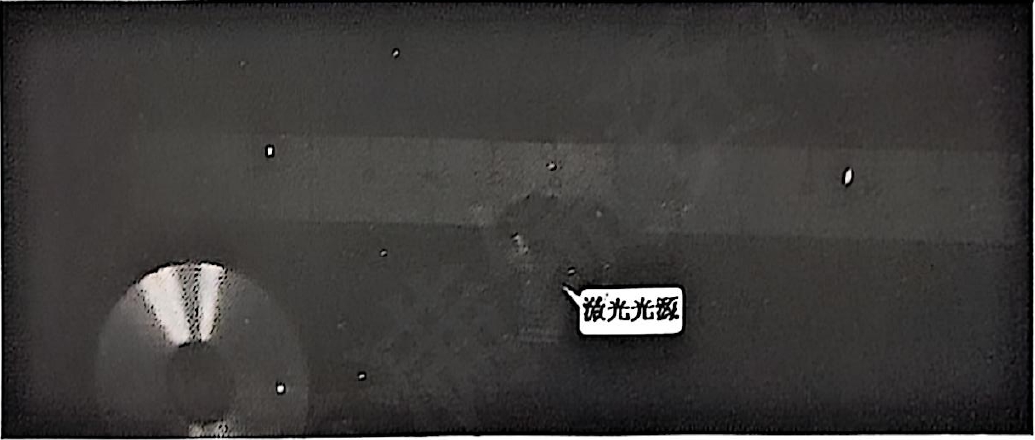
\includegraphics[width=.82\linewidth]{assets/实验照片.png}
\end{center}
\choices{$1050$ 条/$\mathrm{mm}$}{$650$ 条/$\mathrm{mm}$}
{$310$ 条/$\mathrm{mm}$}{$150$ 条/$\mathrm{mm}$}
\end{questionblock}
\begin{questionblock}
\q 利用下列方法测量单色光的波长时，最为准确的是（\quad）。
\choices{双缝干涉}{牛顿环}{单缝衍射}{光栅衍射}
\end{questionblock}
\begin{questionblock}
\q 一束光是自然光和线偏振光的混合光，让它垂直通过一偏振片，若以入射光束为轴旋转偏振片，测得透射光强度最大值是最小值的 3 倍，则入射光束中自然光与线偏振光的光强之比值为（\quad）。
\choices{1}{$1/2$}{$2/3$}{$3/2$}
\end{questionblock}
\begin{questionblock}
\q 光由某种透明介质射向空气时，发生全反射的临界角等于 $45^\circ$，则光从该介质射向空气时的布儒斯特角是（\quad）。
\choices{$35.3^\circ$}{$40.9^\circ$}{$45^\circ$}{$54.7^\circ$}
\end{questionblock}
\begin{questionblock}
\q 如图所示，一束自然光自空气射向一块平板玻璃，设在界面 1 处入射角等于布儒斯特角 $i_{\mathrm B}$，则
\end{questionblock}
\end{document}
